\section{粗盐的提纯}\label{sec:xssy-sy1}

\begin{shiyanmudi}
    初步学会溶解、过滤和蒸发等基本操作。
\end{shiyanmudi}

\begin{shiyanyongpin}
    烧杯、玻璃棒、蒸发皿、酒精灯、漏斗、药匙、量筒(10 毫升)、铁架台(带铁圈)、滤纸、剪刀、托盘天平。

    粗盐。
\end{shiyanyongpin}

\begin{shiyanbuzhou}
    1. 粗盐的溶解 在天平上称取 5 克粗盐(精确至 $0.1$ 克)放在桌上备用。

    \begin{wrapfigure}[16]{r}{5cm}
        \centering
        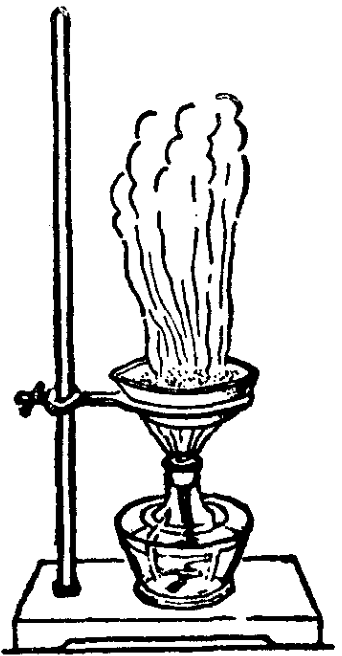
\includegraphics[width=4cm]{../pic/czhx1-xssy-16}
        \caption{蒸发}\label{fig:xssy-16}
    \end{wrapfigure}

    用量筒量取 10 毫升水倒入烧杯里。用药匙取一匙粗盐加入水中,先不搅拌水,观察发生的现象。
    再用玻璃棒搅拌,并观察发生的现象。玻璃棒的搅拌对粗盐的溶解起什么作用?
    接着再加入粗盐,边加边用玻璃棒搅拌,一直加到粗盐不能溶解为止。观察食盐水是否浑浊。

    在天平上称量剩余的粗盐。计算一下在 10 毫升水中约溶解粗盐多少克?

    2. 过滤 按照实验基本操作四所述的方法做一个过滤器,用来过滤食盐水(注意玻璃棒的使用方法)。
    等过滤完毕后,观察滤纸上剩余的物质及滤液的颜色和状态。
    如果滤液还浑浊,应该再过滤一次。观察滤液是否透明。

    3. 滤液的蒸发 把透明的滤液倒入蒸发皿里,再把蒸发皿放在铁架台的铁圈上,用酒精灯加热(图 \ref{fig:xssy-16})。

    在加热过程中,要用玻璃棒不断搅拌液体,以免液体局部过热,致使液滴飞溅出来。
    等到蒸发皿中出现多量固体时,就停止加热。

    4. 固体食盐的洗涤 用玻璃棒把固体移入一个新做的过滤器里,用少量水均匀冲洗,洗掉固体表面残留的液体。

    把制得的食盐跟原来的粗盐进行比较,然后把食盐倒在教师指定的容器里。
\end{shiyanbuzhou}

\begin{wentihetaolun}

    1. 根据实验中得到的数据,估算在 100 毫升水中约能溶解粗盐多少克?

    2. 在这个实验里有几个使用玻璃棒的操作,在各个操作中,玻璃棒起的作用有什么不同?

    3. 在进行过滤时要注意哪几点?为什么?

\end{wentihetaolun}
